\section{Results}\label{results}

\subsection{Monte Carlo Outcomes and Temporal Profiles}\label{monte-carlo-outcomes-and-temporal-profiles}

We ran 200 independent simulations for each scenario, introducing probabilistic variation in model parameters as described in Section~\ref{model-description}. Figure~\ref{fig:trajectories} shows the resulting trajectories of global technology \(T(t)\) and available resources \(R(t)\), averaged across runs. These profiles reveal the distinct collapse and recovery dynamics that characterize each scenario. As expected, Golden Age (S3) and Out of Eden (S10) show uninterrupted growth and resource stability throughout the 1000-year window, consistent with their post-scarcity narratives and reflected in perfect duty cycles (\(\overline{D}_c = 1.0\)) and no collapse events (\(\overline{N}_c = 0\)). In stark contrast, scenarios such as Big Brother (S1) and Sword of Damocles (S6) suffer early collapses (\(\overline{T}_c < 210\)) and high collapse frequency (\(\overline{N}_c \approx 4.5\) for S6 and nearly 10 for S1), leading to sharp contractions in technological capacity and prolonged periods of inactivity. Deus Ex Machina (S9), although collapsing later (\(\overline{T}_c \approx 689\)), also experiences multiple interruptions and never recovers full continuity, with only modest duty cycle (\(\overline{D}_c \approx 0.91\)) and about 1.5 collapse events on average.

\begin{figure*}[htbp]
\centering
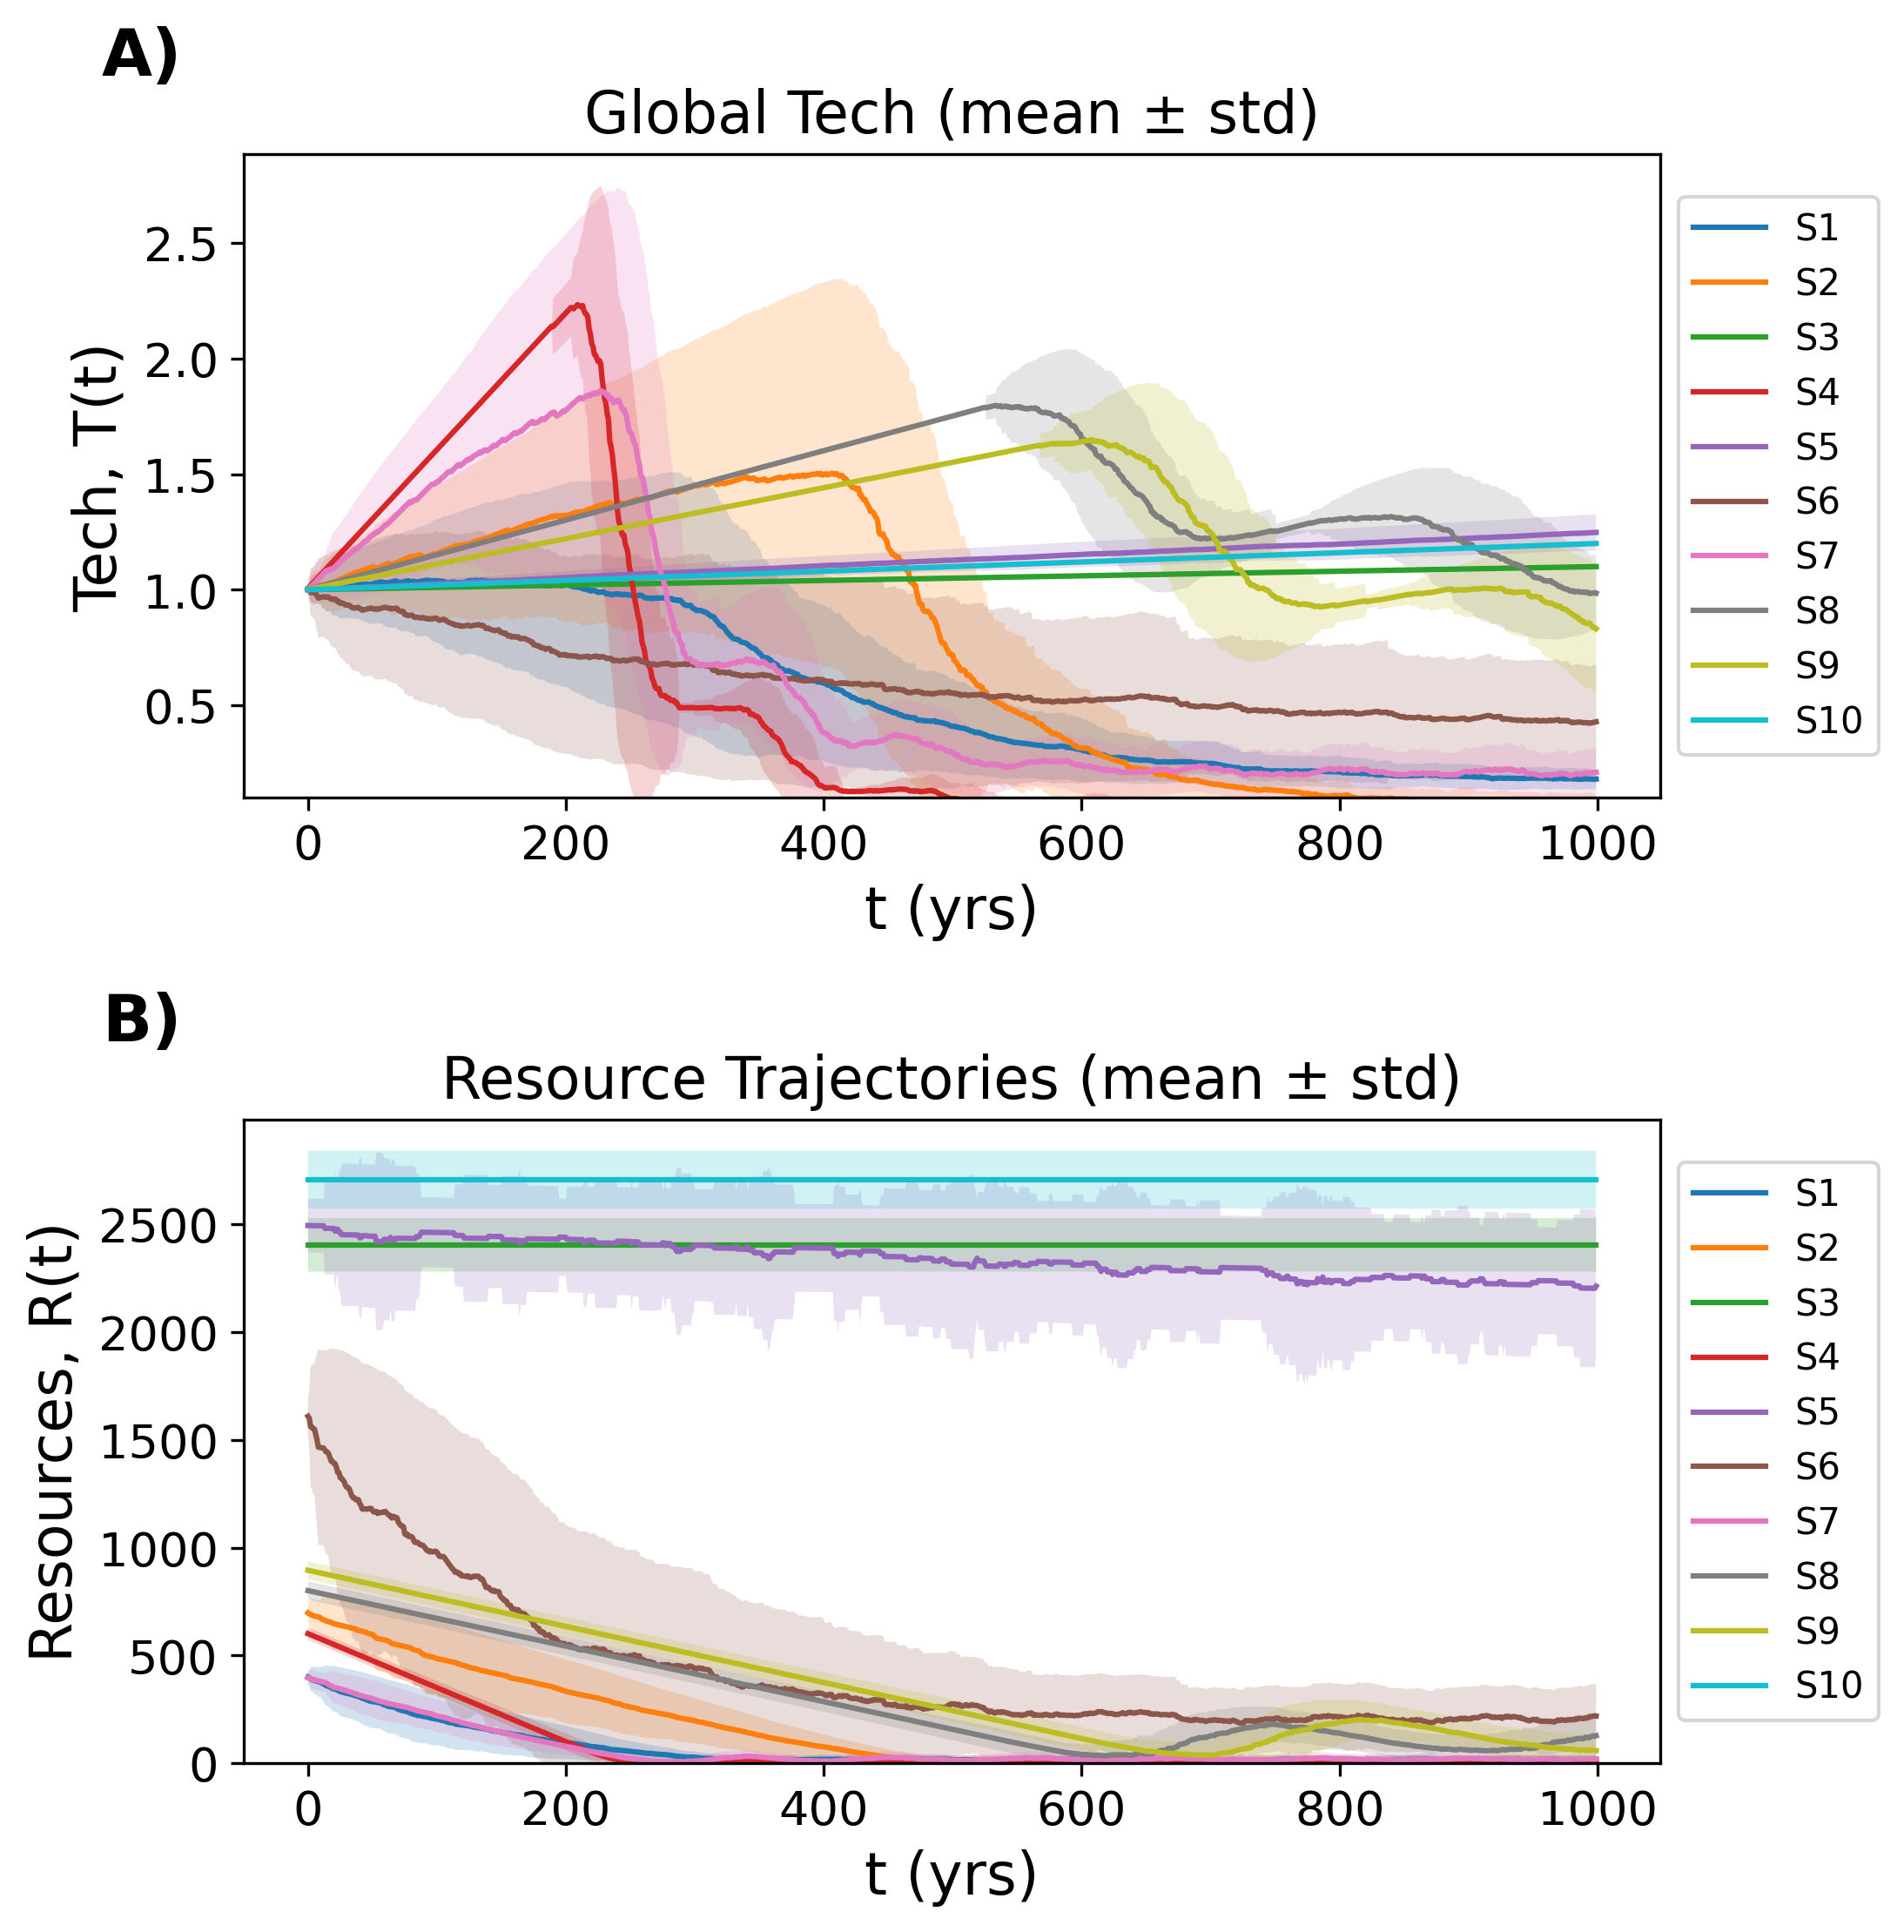
\includegraphics[width=0.7\textwidth]{../figures/tech_and_resources.png}
\caption{Temporal dynamics of simulated civilizations across ten scenarios. (A) Mean trajectories of global technology \(T(t)\) with $\pm 1$ standard deviation shaded. (B) Mean resource levels \(R(t)\) with $\pm 1$ standard deviation shaded.}
\label{fig:trajectories}
\end{figure*}

More complex dynamics emerge in intermediate cases. Transhumanism (S5) avoids collapse in roughly two-thirds of runs and achieves a near-continuous duty cycle (\(\overline{D}_c \approx 0.99\)), albeit with slower growth and occasional extinction. Living with the Land (S4), in contrast, undergoes frequent and deep collapses (\(\overline{N}_c \approx 6.6\)), producing the lowest sustained activity among all non-terminal scenarios (\(\overline{D}_c \approx 0.38\)) despite a steep initial growth phase. Restoration (S7), designed as a post-collapse recovery regime, displays consistent rebuilding behavior: early collapses (\(\overline{T}_c \approx 223\)), followed by approximately 7.5 recovery cycles and moderate continuity (\(\overline{D}_c \approx 0.57\)). Ouroboros (S8) exhibits a distinct pattern of low-frequency, self-stabilizing oscillations: it collapses only twice on average, yet maintains robust technological levels and a high duty cycle (\(\overline{D}_c \approx 0.87\)), reflecting a regime that cycles gracefully without exhausting resources or triggering runaway collapse.

Because the S8 narrative implies repeated collapse--recovery cycles, we ask whether those oscillations are always transient or can be sustained; we probe this with a sweep over $r_f$ and $\delta$ (Figure~\ref{fig:s8sweep}). Panel~A shows deterministic technology trajectories for varying $r_f$ while holding all other S8 parameters at their baseline values. For low recovery fractions ($r_f \leq 0.15$), the system undergoes rapid, repeated collapse--recovery cycles (3 cycles within the 1000-year window), as the diminished resource base after each recovery is quickly exhausted. At intermediate values ($0.20 \leq r_f \leq 0.50$), the system sustains two collapse--recovery cycles with longer growth phases between collapses. At higher recovery fractions ($r_f = 0.60$), the first collapse is delayed significantly, and only a single cycle occurs within the simulation window. Panel~B maps the number of collapse cycles across the $(r_f, \delta)$ parameter space, revealing a clear regime boundary: high depletion rates combined with low recovery fractions produce the most frequent oscillations (up to 8 cycles), while low depletion and high recovery fractions suppress collapse entirely. The baseline S8 parameters (marked with a star) sit near the boundary between 2- and 3-cycle regimes, suggesting that modest shifts in resource recovery capacity could qualitatively alter the civilization's long-term trajectory. These results confirm that S8's oscillatory behavior is not universally stable and it depends sensitively on the balance between resource depletion and post-collapse recovery, with some parameter combinations producing sustained cycling and others leading to dampened or terminal collapse.

\begin{figure*}[htbp]
\centering
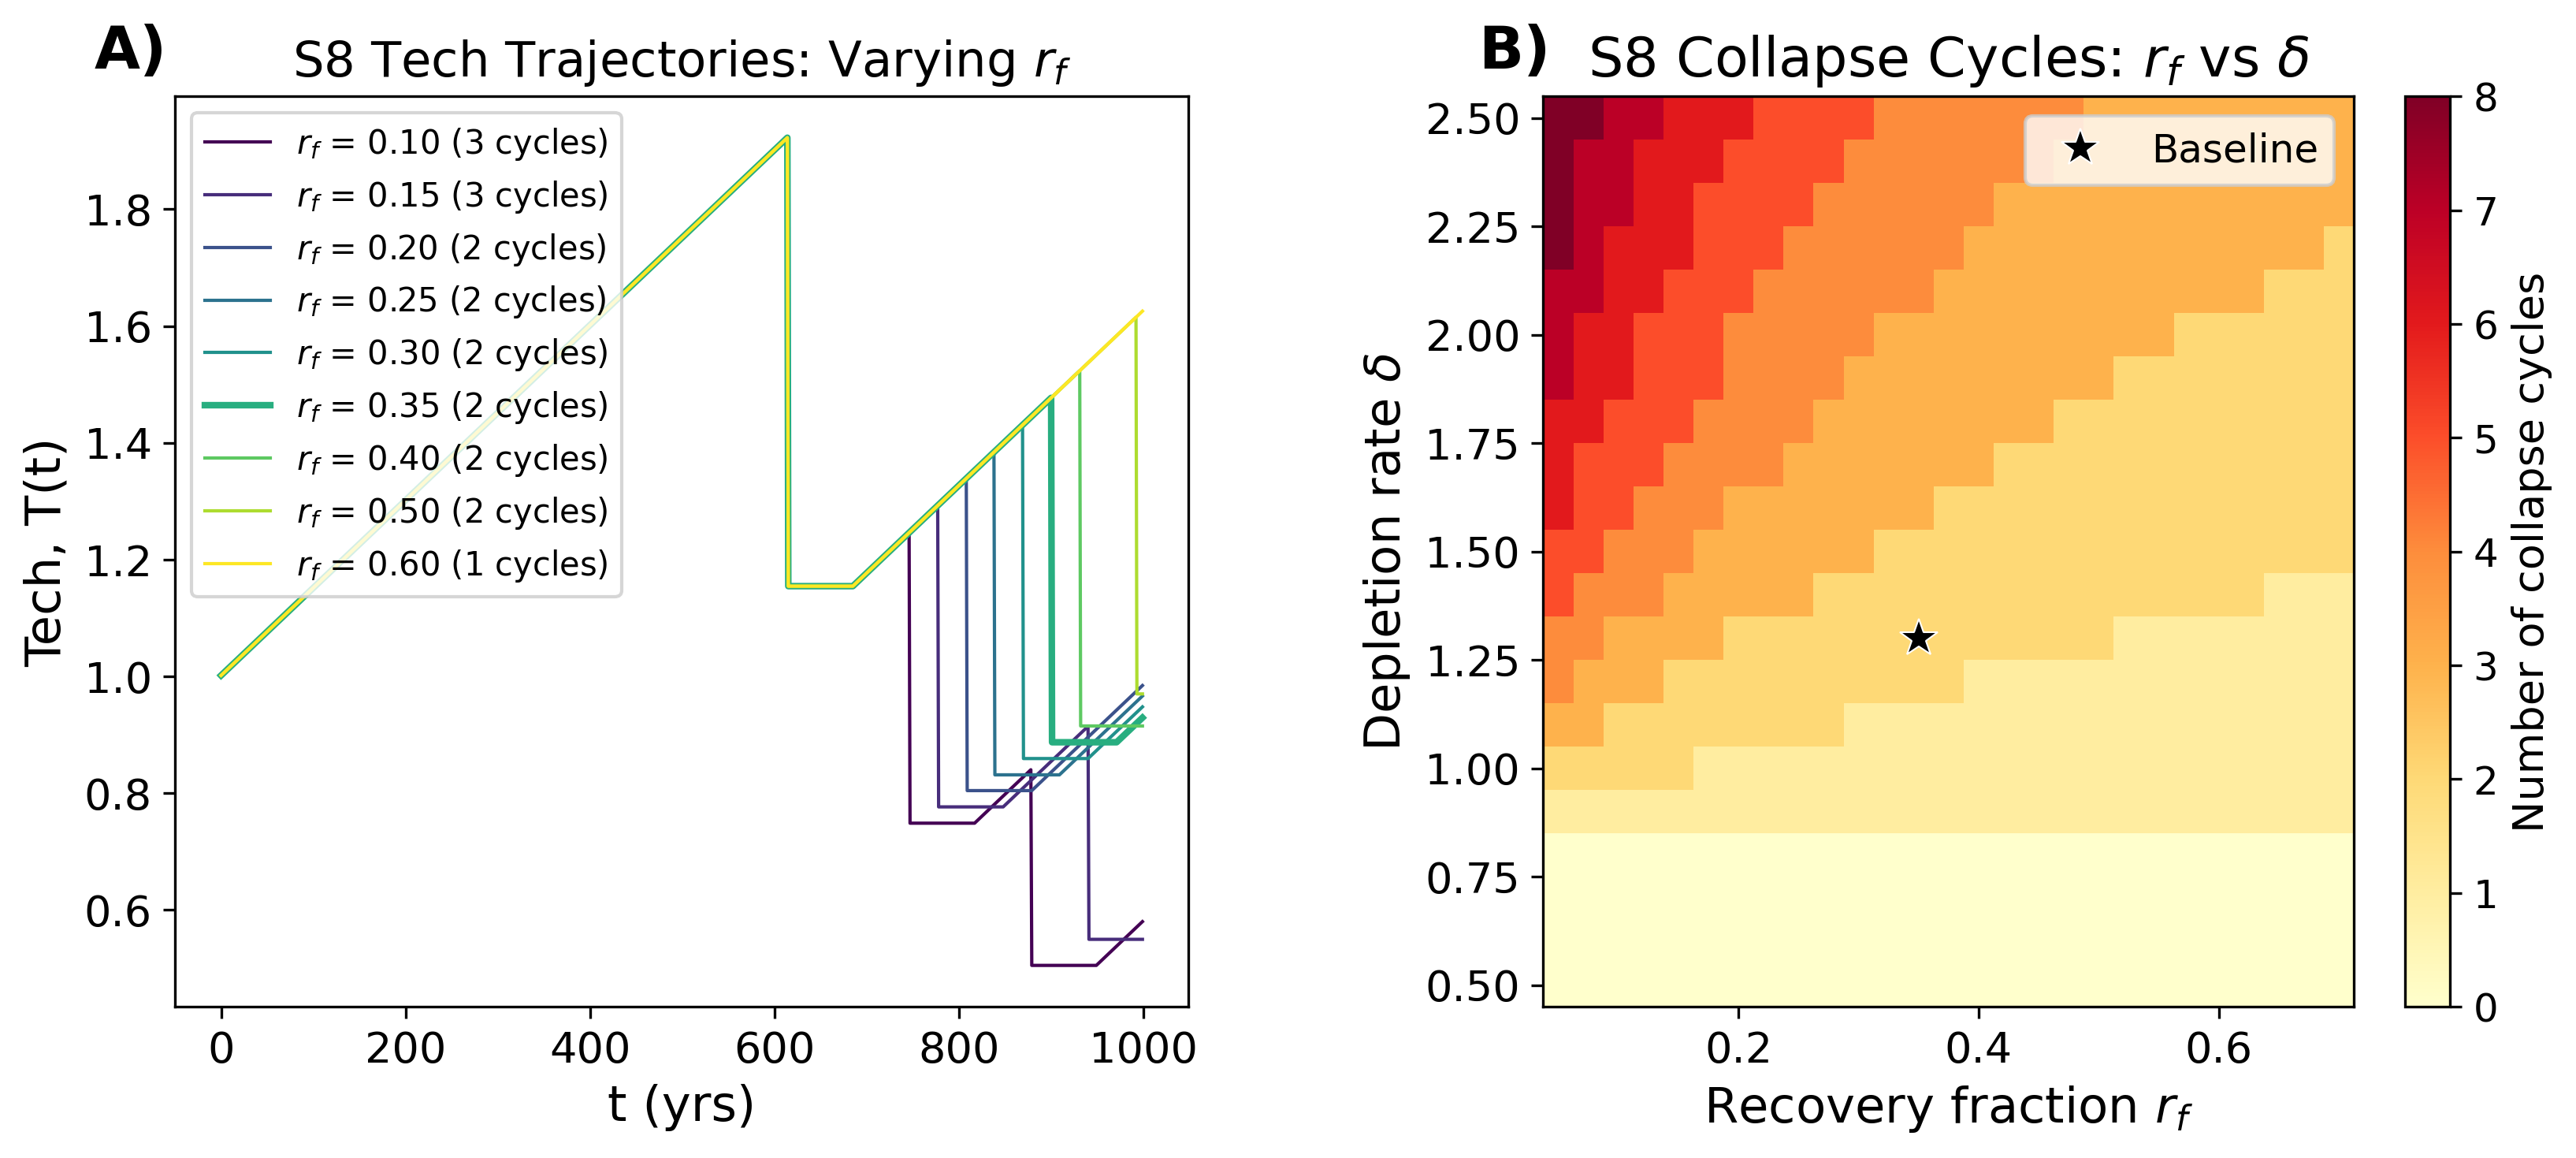
\includegraphics[width=\textwidth]{../figures/s8_parameter_sweep.png}
\caption{Parameter sensitivity of S8 (Ouroboros) oscillatory dynamics. (A)~Deterministic technology trajectories $T(t)$ for varying recovery fraction $r_f$, with all other parameters held at baseline values. The number of collapse--recovery cycles within the 1000-year window is indicated in the legend. (B)~Number of collapse--recovery cycles as a function of recovery fraction $r_f$ and depletion rate $\delta$. The star marks the baseline S8 parameter combination.}
\label{fig:s8sweep}
\end{figure*}

Figure~\ref{fig:metrics} summarizes the outcomes of these simulations using the four metrics described above (\(\overline{T}_c\), \(f_{nc}\), \(\overline{D}_c\), \(\overline{N}_c\)). The scenarios divide into two distinct groups. S3, S5, and S10 survive the full 1000-year window in most or all runs (\(f_{nc} \geq 0.66\); Figure~\ref{fig:metrics}A), maintaining continuous or near-continuous technological activity (\(\overline{D}_c \geq 0.99\); Figure~\ref{fig:metrics}B). In contrast, the remaining seven scenarios collapse in every run, with S1 and S6 breaking down within the first 200 years on average (Figure~\ref{fig:metrics}C). Among the collapse-prone scenarios, the duty cycle spans a wide range---from 0.381 for S4 to 0.91 for S9---reflecting very different recovery capacities despite universal collapse. The most cyclical scenarios are S1 and S7, which undergo roughly 10 and 7.5 collapse--recovery cycles respectively (Figure~\ref{fig:metrics}D), while S8 cycles only about twice, consistent with its low-frequency oscillatory regime.

\begin{figure*}[t]
\centering
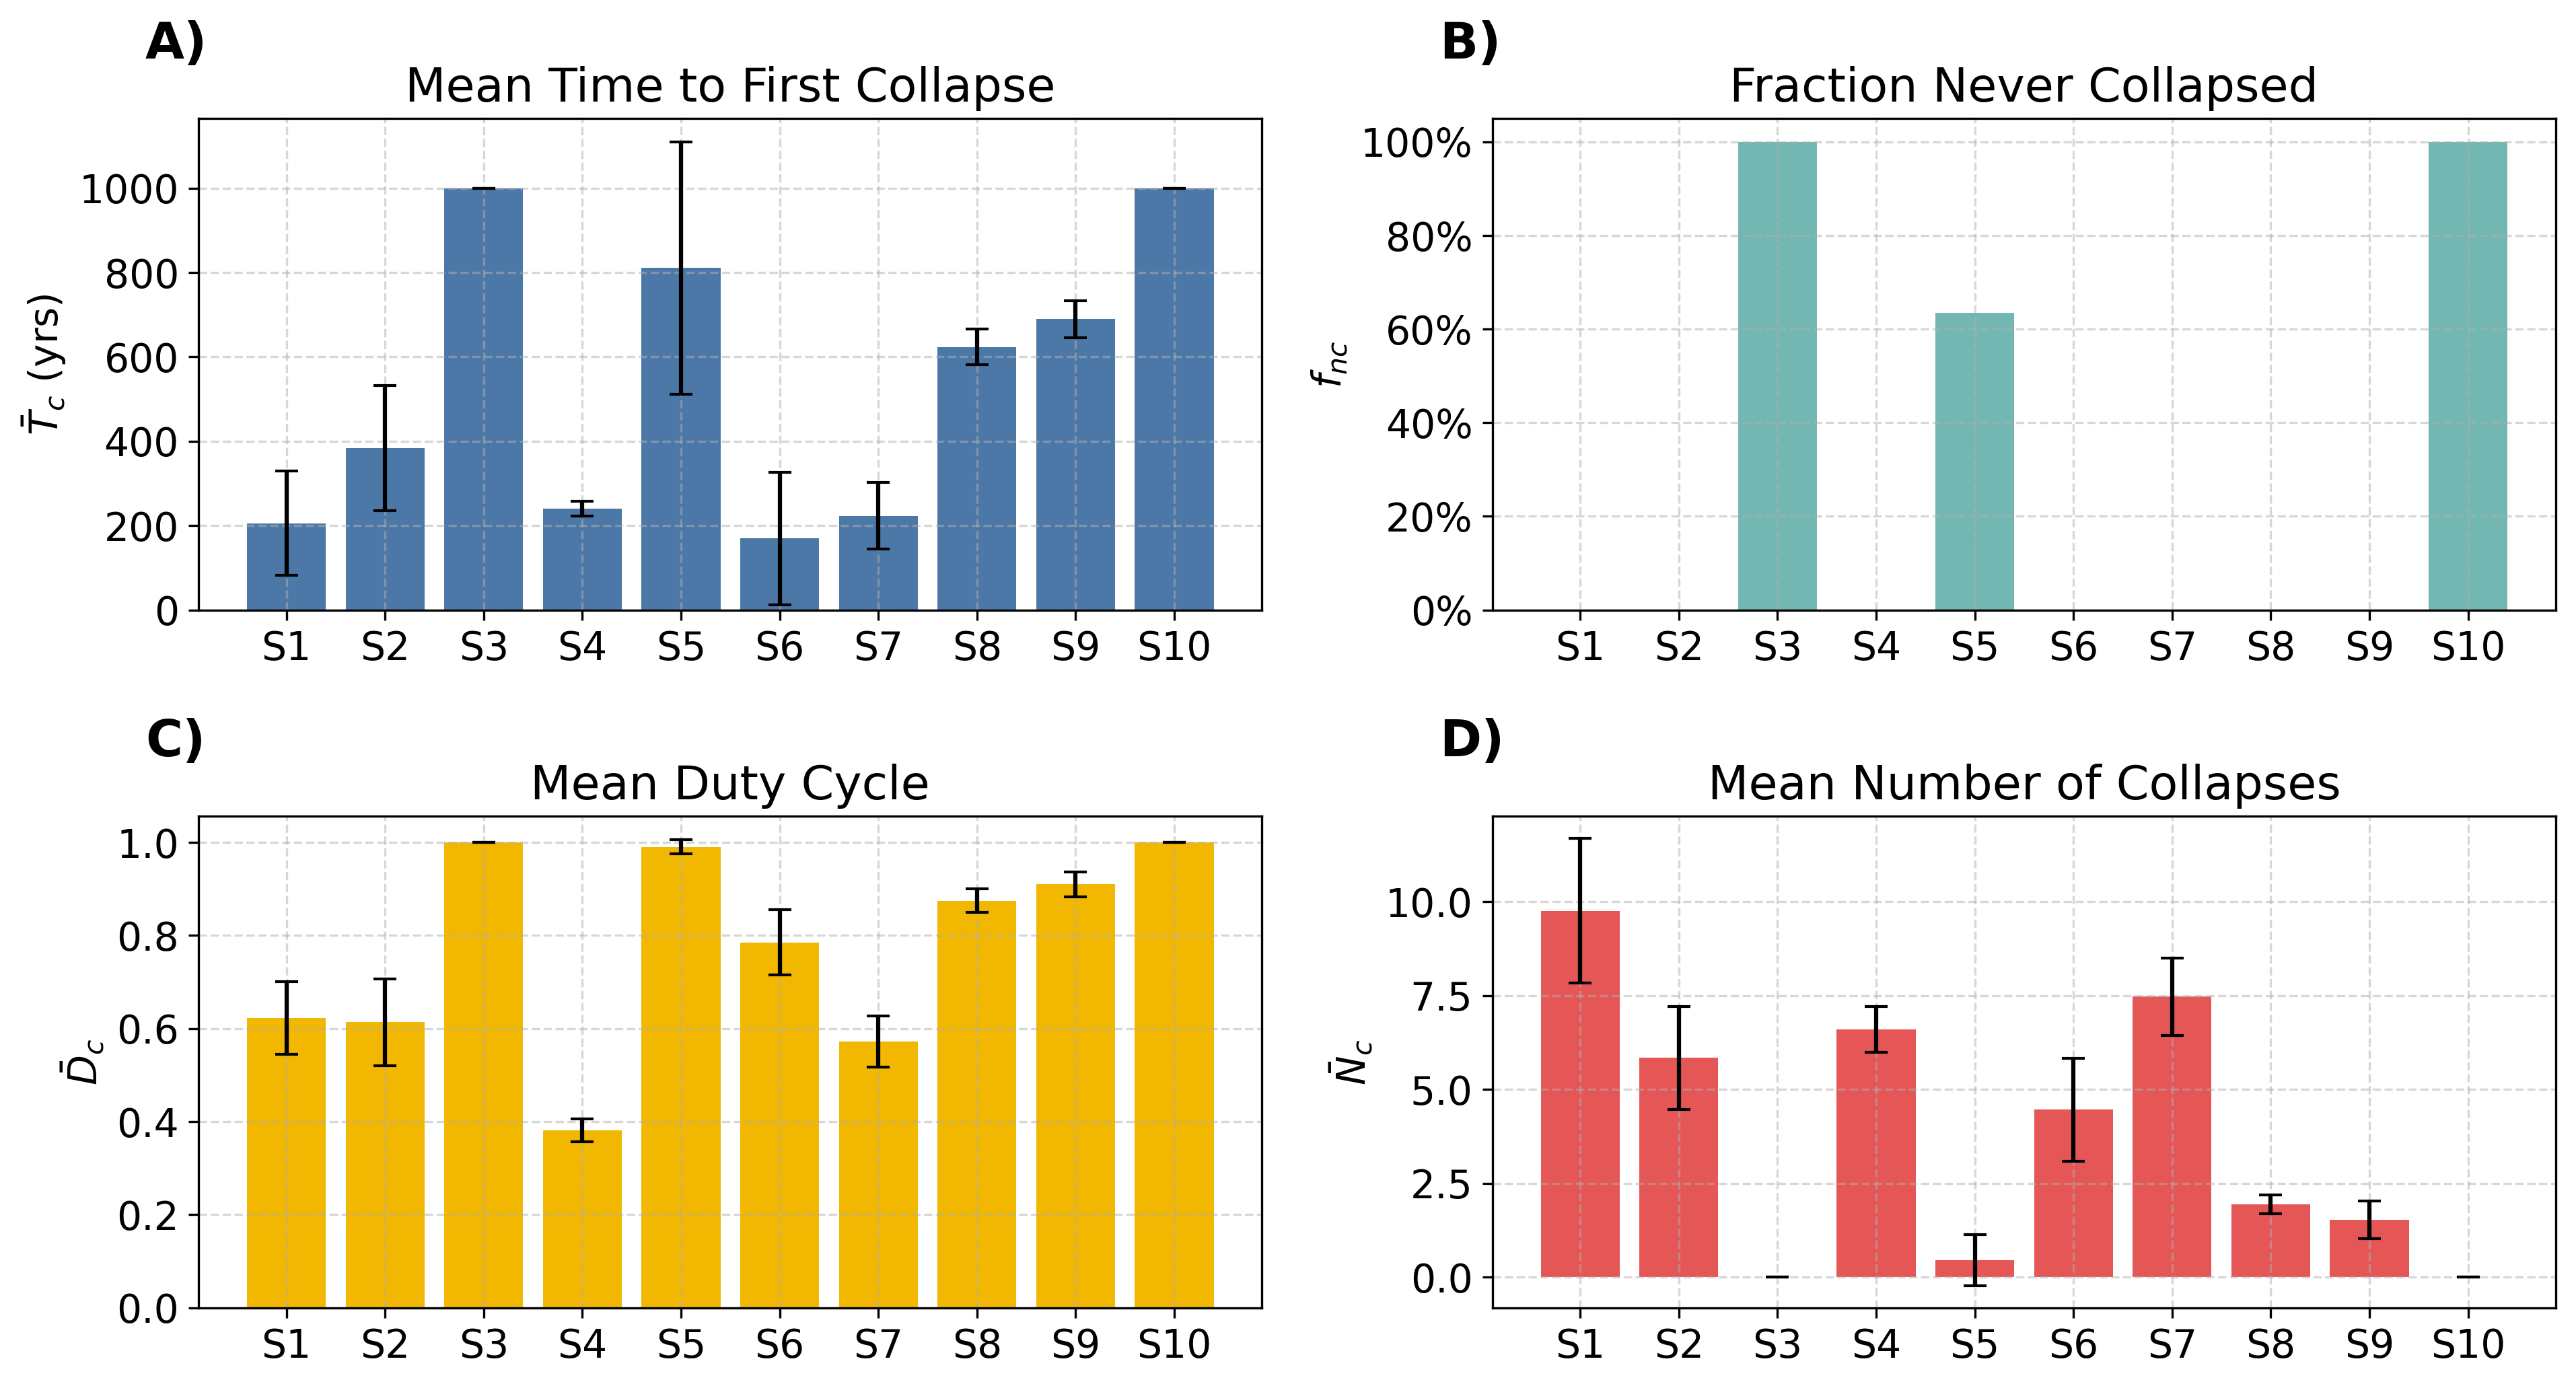
\includegraphics[width=\textwidth]{../figures/summary_panel.png}
\caption{Distributions of key collapse and recovery metrics across scenarios (200 runs each). (A) Fraction of simulations that never experienced collapse \(f_{nc}\). (B) Mean duty cycle \(\overline{D}_{c}\), defined as the fraction of time the technosphere remains active. (C) Mean time to first collapse \(\overline{T}_{c}\) with standard deviation bars. (D) Mean number of collapse events \(\overline{N}_{c}\).}
\label{fig:metrics}
\end{figure*}
